\section{Introduction}

In this chapter, we aim to uncover the underlying principles that govern the stability of a given switch. To do this, we developed an algorithm, called StabilityFinder, that can find the parameter value ranges that can produce the desired stability in a given model. We use this algorithm to examine a variety of switch architectures using different modelling abstractions.

Structurally, this chapter is organised as follows: In the first section we examine the current understanding of the stability landscape of the genetic toggle switch. Then, we discuss the development of StabilityFinder, justify the choices made and the drawbacks of this method. In the sections following we apply StabilityFinder to a variety of models and finally we discuss the implications our findings have to the overall understanding of the toggle switch stability. 

%\section{Parameter scan}
%\subsection{Background}
%
%    
%\subsection{Methods}
%
%\par
%A scan of the parameter values and initial species concentrations of the general toggle switch (shown in Figure~\ref{fig:Toggle switch example}) was performed in this work. This illustrated the presence of tristable, bistable and monostable systems given a different set of parameter values. In addition, the scan was carried out to identify a set of parameter values that leads to a bistable system with maximum distance between the two steady states. This system is able to produce high amounts of the response protein when switched on. A symmetric model, where the parameters for equivalent reactions were set to be the same, was used for simplicity. The algorithm of the scans is outlined below:
%
%\begin{algorithm}[H]
%	\label{alg:param_scan}
%  \caption{Parameter scan}
% \begin{algorithmic}[1]
%    \Statex
%	\State Sample parameters from $U(0, 10)$
%	\ForAll{Sample}
%    	\State Sample initial conditions via Latin Hypercube sampling~\autocite{Mckay:2000lhs}
%    	\ForAll{Samples}
%    		\State Simulate model
%    		\State Solve to steady state
%    	\EndFor
%    \EndFor
%  \end{algorithmic}
%\end{algorithm}
%
%%\begin{itemize}
%%\item Select multiple sets of parameter values from a random uniform distribution between 0 and 10.
%%\item For each set of parameter values:
%%    \begin{itemize}
%%    \item Select multiple sets of initial conditions for the two dimers via latin hypercube sampling:
%%    The space from which the sampling will take place, here between 0 and 10 for both species, is divided equally into 100 smaller subspaces and one value is selected from each subspace~\autocite{Mckay:2000lhs}. Therefore it is ensured the whole space is sampled from. 
%%    \item For each set of initial conditions:
%%        \begin{enumerate}
%%        \item Integrate ODEs of the model
%%        \item Solve system to steady state
%%        \end{enumerate}
%%    \end{itemize}
%%\end{itemize}
%
%
%
%One dimer was plotted against the other for all initial conditions of each parameter set. An example for each of the three types of stabilities found during the scan are shown in Figure~\ref{fig:stab exampl}. The parameter sets that resulted in bistability are shown in Table ~\ref{tab: scan params}. 
%
%\subsection{Results}
%\begin{figure}[h!]
%\centering
%\includegraphics[scale=0.9]{chapterStabilityFinder/images/switch_stbility_examples.pdf}
%\captionof{figure}{An example for each type of switch found during the parameter scan. Each graph represents the steady state values of one dimer plotted against the other, from one parameter set and 100 initial conditions.}
%    \label{fig:stab exampl}
%\end{figure}
%
%In order to determine which areas in the parameter space give rise to the different kinds of stability, a histogram of the frequency of each parameter value found in monostable, bistable and tristable systems was plotted and shown in Figure~\ref{fig:scan ode param hist}.
%
%
%\begin{figure}
%\centering
%\begin{minipage}[c]{1\textwidth}
%\centering
%    \includegraphics[width=1.05\textwidth]{chapterStabilityFinder/images/param_stability_hist.pdf}
%    \caption{The distribution of parameter values that resulted in monostable, bistable and tristable switches in the parameter scan. Each graph represents the distribution of the values of one parameter. }
%    \label{fig:scan ode param hist}
%\end{minipage}
%\end{figure}
%
%
%
%\begin{table}[h!]
%\centering
%\caption {The parameter values obtained from the parameter scan that resulted in bistability. Each row corresponds to a set of parameter values.} \label{tab: scan params}
%\begin{tabular}{ccccccc}
%\toprule
% \textbf{ge}     & \textbf{rep}    & \textbf{rep r}     & \textbf{dim}    & \textbf{dim r}     & \textbf{deg      }\\
% \midrule
%6.95   & 9.53    & 1.890     & 6.43   & 7.06      & 2.91   \\
%4.82   & 4.37    & 0.595     & 9.45   & 2.07      & 3.72   \\
%8.44   & 6.53    & 0.818     & 8.15   & 3.59      & 9.99   \\ 
%6.46   & 7.92    & 2.650     & 3.07   & 8.01      & 1.91   \\
%8.15   & 9.42    & 1.44      & 6.13   & 5.45      & 4.84     \\
%8.89   & 8.98    & 5.39      & 3.56   & 7.39      & 2.24     \\
%8.01   & 9.95    & 5.69      & 5.95   & 4.01      & 1.90     \\
%6.28   & 4.88    & 2.11      & 4.96   & 2.44      & 4.24     \\
%9.48   & 9.40    & 3.69      & 2.16   & 3.95      & 2.08     \\
%7.72   & 6.19    & 2.31      & 5.97   & 1.58      & 5.40     \\
%3.60   & 3.80    & 0.43      & 8.90   & 4.66      & 2.24     \\
%8.23   & 4.31    & 2.07      & 7.94   & 3.52      & 6.32     \\
%9.36   & 7.33    & 7.47      & 8.19   & 9.87      & 2.99   \\
%8.16   & 2.08    & 1.36      & 3.29   & 8.27      & 1.62   \\
%8.52   & 8.09    & 4.41      & 4.25   & 1.23      & 6.48   \\
%8.15   & 4.42    & 1.05      & 5.44   & 9.57      & 2.16   \\
%\bottomrule
%\end{tabular}
%\end{table}   
%   
%\clearpage
%\subsection{Discussion}
%\par
%   The parameter scan was successfully completed in the deterministic case and some of the results shown in Figure \ref{fig:stab exampl}. Different parameter sets resulted in different stability of the toggle switch.   
%     
%\par
%   There were a total of 217 monostable, 16 bistable and 6 tristable switches out of 400 sampled parameter sets. The remaining samples did not reach steady state. This shows that different parameter values have a great effect on the stability profile of the switch. Note the symmetry of the steady states of each bistable switch is due to the use of a symmetric model. 
% 
%\par 
%    Some interesting results arise from the histograms in Figure ~\ref{fig:scan ode param hist}. It can be seen that the parameter for gene expression (ge) tends to be relatively high when bistability arises whereas the parameter for the reverse reaction of repression (rep r) tends to be low. Degradation (deg) also tends to be low. It must also be noted that the parameter values that give rise to monostable systems are generally evenly distributed for all parameters, suggesting that monostable systems arise from the whole range of values sampled. This can further indicate that the right combination of more than one parameter values is necessary for bistability. Further analysis is thus needed to determine what these combinations are. A sensitivity analysis of the model will be carried out in order to determine which parameters affect bistability and to which parameters is the system robust. The parameter scan will also be incorporated into the ABC SMC methodology, in order to identify the parameter values required for bistability more efficiently.             
%
%\par
%    In this work it was shown that a range of stability profiles are achievable by the standard toggle switch. The patterns of the parameter values required for each are beginning to emerge. Further work is required in order to get a definitive answer for the stability characteristics of the toggle switch given this modelling approach.
%
%\section{Bayesian approach to model stability}
\section{Background}
Synthetic biology is now entering an age where simple synthetic circuits have been built, such as toggle switches \autocite{Gardner:2000vha, Kramer:2004kq, Isaacs:2003ht, Ham:2008hh, Deans:2007cya, Friedland:2009ce}, oscillators~\autocite{Stricker:2008jqa, Fung:2005jd, Tigges:2009jx} and pulse generators~\autocite{Basu:2004gn}, but larger circuits have proven more difficult \autocite{XXX}. The leap from building low-level circuits to assembling them into complex networks has yet to be made successfully~\autocite{Lu:2009ez}, and predictable circuit behaviour remains challenging \autocite{XXX}. Efforts to do so are plagued by intra-circuit crosstalk and incompatibility, as well as cellular noise, which can render synthetic networks non-functional \textit{in vivo} \autocite{XXX}. 

A circuit must be robust to a fluctuating cellular environment and its response and sensitivity must be able to be fine tuned in order to orchestrate a network of circuits that function together. A robust circuit can tolerate the compound stochasticity that a chain of circuits brings, and fine tuning of its response and sensitivity enables the researcher to make it sensitive to an upstream signal as well as influence a downstream subsystem. Parts can be fine tuned by developing component libraries~\autocite{Lu:2009ez,}, but this will be of little use if the required parameter ranges for parts to make a functional complex network are unknown, and will only perpetuate the cycles of trial-and-error. A computational method to find the range of parameter values that will produce the behaviour of choice is crucial to the design process by enabling the informed selection of appropriate parts from the libraries. If it is known that gene expression must be low for a given stability, one can select a weak promoter or a low copy plasmid for the desired construct. 

Both analytical and computational approaches have been deployed for the study of the toggle switch. Analytical approaches are limited to simpler models and thus require a number of assumptions to be made. The system under consideration has to be reduced to very few equations and parameters in order to make the system solvable. This requires assumptions to be made about the system that cannot always be justified, such as the quasi-steady state approximation (QSSA). The QSSA assumes that the binding/unbinding processes are much faster than any other process~\autocite{Loinger:2007vma}, thus the bound intermediate is assumed to always be in steady state. The QSSA assumption is met \textit{in vitro} but often does not hold \textit{in vivo} and its misuse can lead to large errors and incorrectly estimated parameters~\autocite{Pedersen:2007ke}. Moreover, it is generally not possible to solve even simple stochastic models analytically, and these methods are restricted to deterministic models. The computational and graph-theoretic approaches developed for the study of multistationarity generally focus on deciding on whether a given system is incapable of producing multiple steady states ~\autocite{Conradi:2007jo, Banaji:2010fh,Feliu:2013dz}. For example, ~\textcite{Feliu:2013dz} developed an approach using chemical reaction theory and generalised mass action modelling \autocite{Feliu:2013dz}. No approach exists that can handle both deterministic and stochastic systems in an integrated manner.

Here we present a computational framework based on sequential Monte Carlo that takes a model and determines whether it is capable of producing a given number of (stable) steady states and the parameter space that gives rise to the behaviour. Uniquely, this can be done for both deterministic and stochastic models, and also complex models with many parameters, thus removing the need for simplifying assumptions. Our framework can be used for comparing the conclusions drawn by various modelling approaches and thus provides a way to investigate appropriate abstractions. We have made this framework into a python package, called StabilityFinder. This methodology is used to investigate genetic toggle switches and uncover the design principles behind making a bistable switch, as well as those necessary to make a tristable switch. We find that degradation rates of transcription factors are important for bistability, and that the addition of positive autoregulation can create tristable behaviour and also significantly more robust bistability when feedback strength is well balanced. Modelling transcription and translation allows us to conclude that transcriptional bursting can inhibit bistability, and also that bistability can occur even when the assumptions of time scale separation in the repressor dynamics are not met. We also examine the design principles behind the design of bistable versus tristable switches and highlight the importance of including stochastic dynamics when modelling these systems. Finally we demonstrate the ability of the framework to examine more complex systems and examine the design principles of a three gene switch. These examples demonstrate that StabilityFinder will be a valuable tool in the future design and construction of novel gene networks. 


\subsection{\acrshort{abc} algorithms}

The simplest \acrshort{abc} algorithm is the \acrshort{abc} rejection sampler~\autocite{Pritchard:1999td}. In this method, parameters are sampled from the prior and data simulated thorough the data generating model. For each simulated data set, a distance from that of the desired behaviour is calculated, and if greater than a threshold, $\epsilon$, the sample is rejected, otherwise it is accepted. 
\begin{algorithm}[H]
	\label{alg:ABC}
  \caption{ABC rejection algorithm}
 \begin{algorithmic}[1]
    \Statex
	\State Sample a parameter vector $\theta$ from prior $\pi(\theta)$
	\State Simulate the model given $\theta$
    \State Compare the simulated data with the desired data, using a distance function $d$ and tolerance $\epsilon$. if $d \leq \epsilon$, accept $\theta$ 
   
  \end{algorithmic}
\end{algorithm}


\noindent The main disadvantage of this method is that if the prior distribution is very different from the posterior, the acceptance rate is very low~\autocite{Toni:2009tr}. An alternative method is the \acrshort{abc} \acrfull{mcmc} developed by~\textcite{Marjoram:2003up}~\autocite{Marjoram:2003up}. The disadvantage of this method is that if it gets stuck in an area of low probability it can be very slow to converge~\autocite{Sisson:wf}. 

The method used here is based on sequential Monte Carlo, which avoids both issues faced by the rejection and MCMC methods. It propagates the prior through a series of intermediate distributions in order to arrive at an approximation of the posterior. The tolerance, $\epsilon$ for the distance of the simulated data to the desired data is made smaller at each iteration. When $\epsilon$ is sufficiently small, the result will approximate the posterior distribution~\autocite{Toni:2009tr}.  

The desired behaviour of the system is used as the data to which the candidate model output is compared to \cite{Barnes:2011hh}. Given a set of competing models, their associated prior estimates of their parameters and the design specifications, the algorithm is able to rank the models according to how well they describe the data and the posterior probabilities of the parameters \cite{Barnes:2011hh}. 

ABC SMC can identify the parameter values within a predefined range of values that can achieve the desired behaviour. It works by first sampling at random from the initial range set by the user, i.e. form the prior distribution of values. Each sample from the priors is called a particle. It then simulates the model given those values and compares that to the target behaviour. If the distance between the simulation and the target behaviour is greater than a predefined threshold distance $\epsilon$, then the parameter values that produced that simulation are rejected. This is repeated for a predefined number of samples which are collectively referred to as a population. Each particle in a population has a weight associated with it, which represents the probability of it producing the desired behaviour. At subsequent iterations the new samples are obtained from the previous populations and the $\epsilon$ is set to smaller value, thus eventually reaching the desired behaviour. The algorithm, without model selection, proceeds as follows:

\begin{algorithm}[H]
	\label{alg:ABC-SMC}
  \caption{ABC SMC algorithm}
 \begin{algorithmic}[1]
    \Statex
    \State Select $\epsilon$ and set population t = 0
	\State Sample particles ($\theta$). If t = 0, sample from prior distributions (P). If t $\textgreater$ 0, sample particles from previous population.
	\State If t $\textgreater$ 0: Perturb each particle by $\pm$ half the range of the previous population (j) to obtain new perturbed population (i).
	\State Simulate each particle to obtain time course.
	\State Reject particles if d $\textgreater$ $\epsilon$.
	\State Calculate the weight for each accepted particle. At the first population assign a weight equal to 1 for all particles. In subsequent populations the weight of a particle is equal to the probability of observing that particle divided by the sum of the probabilities of the particle arising from each of the particles in the previous population:

	\State $w_{t}^{(i)} = \begin{cases} 1, & \mbox{if } n = 0 \\\frac{P(\theta_{t}^{(i)})}{\sum_{j=1}^N w_{t-1}^{(j)} K_{t}(\theta_{t-1}^{(j)}, \theta_{t}^{(i)})}, & \mbox{if } n $\textgreater$  0. \end{cases}$

  \end{algorithmic}
\end{algorithm}


This algorithm is implemented on a simple example for illustration. $A$ simple model was used, consisting of one species, $A$ converting to another, $B$. The model is described by two differential equations, where $A$ is the reactant and B the product, produced at a rate $p1$. 

\begin{align*}
\frac {d[B]}{dt} &= p1[A] \\ 
\frac {d[A]}{dt} &= - p1[A] 
\end{align*}

\noindent The priors were set to $p1\sim$U(0, 10). Initial conditions for A and B were set to 1 and 0 respectively. The data to which the model was compared to was generated by simulating the same model with the parameter set to 1, as shown in Figure~\ref{fig:myABC true 1}.

\begin{figure*}[htbp]
    \begin{center}
    \includegraphics[scale=0.6]{chapterStabilityFinder/images/abcsmc_ex.pdf}
    \caption[\acrshort{abc} \acrshort{smc} example]{ABC SMC parameter inference. The posterior parameter is equal to 1 and its time course shown in red in the top left panel. The blue time course is that of the final population, green is the upper quartile and red is the lower quartile range of values. The progress of the selection process can be seen the \textepsilon schedule proceeds from the top left to the bottom right. The bottom far right panel is a density plot of \textepsilon = 0.01 with their weights taken into account.  }
    \label{fig:myABC true 1}
    \end{center}
\end{figure*}
\clearpage


\subsection{Robustness}

{\color{red} Here we define robustness as.. }


{Robustness coming out of Bayesian methods..



\section{Stability Finder algorithm}

The framework is based on a statistical inference method which combines \acrfull{abc} with \acrfull{smc} \autocite{Toni:2009tr}. This simulation-based method uses an iterative process to arrive at a distribution of parameter values that can give rise to observed data or a desired system behaviour \autocite{Barnes:2011hh}.

\acrshort{abc} methods are used for inferring the posterior distribution in cases where it is too computationally expensive to evaluate the likelihood function. Instead of calculating the likelihood, \acrshort{abc} methods simulate the data and then compare the simulated and observed data through a distance function \autocite{Toni:2009tr}. Given the prior distribution $\pi(\theta)$ we can approximate the posterior distribution, $\pi(\theta\mid x)\propto f(x\mid\theta)\pi(\theta)$, where $f(x\mid\theta)$ is the likelihood of a parameter, $\theta$, given the data, $x$. There are a number of different variations of the \acrshort{abc} algorithm depending on how the the approximate posterior distribution is sampled. 

\subsection{Algorithm overview}

To investigate the multistable behaviour of systems, a number of extensions to existing approaches are required. For a given set of parameter values, sample points are taken across initial conditions using latin hypercube sampling \autocite{XXX}, and the ensemble system simulated in time until steady state. The distance function in \acrshort{abc} is replaced by a distance on the desired stability of the simulated model. To do this we cluster the steady state coordinates using Kmeans clustering and use the gap statistic to determine the number of clusters \autocite{XXX}. The algorithm is summarised below.

\begin{algorithm}[H]
\label{alg:StabilityFinder}
\caption{StabilityFinder algorithm}
 \begin{algorithmic}[1]
    \Statex
	\State Initialise $\epsilon$ 
	\Let{population p}{1}
	\If{p $= 1$}
		\State Sample particles ($\theta$ ) from priors
		\Else
			\State Sample particles from previous population
			\State Perturb each particle by $\pm$ half the range of the previous population (j) to obtain new perturbed population (i).
	\EndIf
	\State Sample initial conditions via Latin Hypercube Sampling.
    \State Simulate each particle to obtain steady state values.
    \State Cluster steady state
	\State Reject particles if d $\textgreater$ $\epsilon$.
    \State Calculate weight for each accepted $\theta$
	%\State $w_{t}^{(i)} = \begin{cases} 1, & \mbox{if } p = 0 \\\frac{\pi(\theta_{t}^{(i)})}{\sum_{j=1}^N w_{t-1}^{(j)} K_{t}(\theta_{t-1}^{(j)}, \theta_{t}^{(i)})}, and \mbox{if } p \geq  0. \end{cases}$
	\State Normalise weights
	\Repeat{steps 3 - 15} \Until{$\epsilon \leq \epsilon_T$}
  \end{algorithmic} 
\end{algorithm}

\noindent This algorithm is available as a Python package, called StabilityFinder. %which is available at \url{https://github.com/ucl-cssb/StabilityFinder.git}.  

The user provides an SBML model file \autocite{XXX} and an input file that contains all the necessary information to run the algorithm, including the desired stability and the final tolerance, \textepsilon, for the distance from the desired behaviour necessary for the algorithm to terminate. The flow of execution is illustrated in Figure~\ref{fig:fig1}. Since the algorithm is computationally intensive, all deterministic and stochastic simulations are performed using algorithms implemented on \acrfull{gpu}s \autocite{XXX}.

\begin{figure*}[h]
\begin{center}
\includegraphics[scale=0.9]{chapterStabilityFinder/images/SF_algo_overv.png}
\caption[LoF caption]{\label{fig:fig1}: Using sequential Monte Carlo to examine system stability. The algorithm takes as input a model (A) and evolves it to the stability of choice (C) via intermediate populations. In this example model shown in A, There are two species and two parameters. For the model to be bistable, the phase plot of the two species of interest must have two distinct densities, as shown in (C). The parameter space of the model is searched through our algorithm until the resulting simulations give rise to bistability. The parameter values for the model that demonstrated the desired behaviour are given as an output (D). The output consists of the accepted values for each parameter, as well as each density plotted against the other. This allows us to uncover correlations between parameter values. We made this algorithm into a python package, called Stability Finder. The overview of the algorithm is shown in (E).}
\end{center}
\end{figure*}
\clearpage


\begin{figure*}[h]
\begin{center}
\includegraphics[scale=0.5]{chapterStabilityFinder/images/process_overv.png}
\caption[LoF caption]{q}
\end{center}
\end{figure*}
\clearpage

\subsection{Particle sampling}
For the first population, particles are sampled from the priors. Random samples are taken from the distribution specified by the user for each parameter. 

For subsequent populations particles are sampled from the previous population. The weight of each particle in the previous population dictates the probability of it being sampled. Using Bernouli trials.

\subsection{Perturbation}
Each sampled particle is perturbed by a kernel defined by the distribution of the previous population. 

\begin{align*}
K_p(\theta|\theta* ) &= \theta* + U(+s_p, -s_p) \\
s_p &= \frac{1}{2} \big (max(\theta_{p-1}) - min(\theta_{p-1}) \big ),
\end{align*}

If the \texttheta* falls out of the limits of the priors then the perturbation is rejected and repeated until an acceptable \texttheta* is obtained. The drawback of this perturbation kernel is that it can be computationally costly.
\subsection{Initial condition sampling}

In Stability Finder, latin hypercube sampling is used to sample initial conditions (XXX). This is used to ensure that the whole space is sampled evenly. Latin hypercube sampling is done in two dimensions in Stability Finder. The uniform priors of the two species in consideration represent a rectangle space, which is subdivided into equal parts. Then a random sample is drawn from each sub-part. This ensures the whole space is evenly sampled. 

\begin{figure*}[htbp]
\begin{center}
\includegraphics[scale=0.5]{chapterStabilityFinder/images/LHS.png}
\caption[LoF caption]{\label{fig:lhs}Latin Hypercube Sampling}
\end{center}
\end{figure*}

Stability Finder can only be used for stability analysis concerning two species. By that I refer to models where the phase plot is always and only two-dimensional. Stability landscapes involving more that two species are beyond the scope of this thesis. 
\clearpage
\subsection{Particle simulation}

Each particle is simulated using cudasim (XXX). Cudasim is 

\subsection{Distance function}
 
 The distance function is the function the algorithm uses to compare the desired behaviour to the behaviour observed in each particle (XXX). In StabilityFinder the distance function consists of three distances. The first one is the difference between the number of desired clusters and the number of clusters observed in the phase plot. For this distance metric the number of clusters in the phase plot must be calculated. The clustering methods used are outlined in section~\ref{Clustering methods}.
 
 The other two distance metrics used in StabilityFinder are the variance within each cluster and the overall variance. The within-cluster variance ensures that the clusters are tight, and the between-cluster variance is used to ensure the clusters are far apart from each other. The ideal behaviour of a system we seek is tight, widely separated clusters. This means that the genetic system has two distinct steady states, and the difference in the protein levels are observable.
 
\subsubsection{Clustering methods}
\label{Clustering methods}

Whether the model was simulated using \acrshort{ode}s or the Gillespie algorithm dictated the method of clustering that we used. For the deterministic models I used an algorithm I developed, that will be referred to as the Delta clustering algorithm in this thesis. This algorithm consisted of defining the number of clusters by counting a new cluster every time a data point is more than a distance delta away from any existing clusters. The benefits of the Delta clustering algorithm are that it is fast and can be used on deterministic solutions, where steady state values tend to be identical if all the particles have reached steady state (XXX).

Steady states of stochastic models are clustered using the K-means clustering (XXX) and the number of clusters determined using the Gap statistic (XXX). This method is more suited to stochastic solutions, where the Delta clustering method would fail as the steady state solutions tend to be more widely dispersed than in the deterministic case. 

The method used for clustering can be altered by the user if he/she wants to add their own preferred clustering algorithm more appropriate for their specific purposes. For the models we used here, the above methods were successful in clustering the steady state solutions. 

\subsection{Particle rejection}

A particle can be rejected for any number of the following reasons:
\begin{enumerate}
	\item Particle cluster distance \textgreater \textepsilon\textsubscript{c}
	\item Particle V\textsubscript{bc} distance \textgreater \textepsilon \textsubscript{Vbc}
	\item Particle V\textsubscript{wc} distance \textgreater \textepsilon \textsubscript{Vwc}
	\item Particle SS\textsubscript{v} \textgreater \textepsilon \textsubscript{ssv}
	\item Particle SS\textsubscript{l}  \textgreater \textepsilon \textsubscript{ssl}
\end{enumerate}


I included a check for whether the model simulation had reached steady state. If the standard deviation of the last ten time points in the simulation is larger than a user-specified value (default is set to 0.0001), then the particle is rejected. This is to ensure that only particles that have reached steady state are considered. 

\subsection{Weight calculation}

The weights of the particles are calculated by considering the previous population. The numerator $\prod_{p=1}^{R} (max(perturbation) - min(perturbation))^{-1}$. The denominator is.

The weights are then normalised over the total number of particles. 
    

\subsection{Model checking}

A problem that can arise by using this method with stochastic simulations is that the behaviour observed may not be the true behaviour but it might be a result of noise. We need to ensure that the resulting behaviour is reproducible. Therefore, I added model checking to the algorithm. Model checking consists of resampling from the posterior distribution and simulating each sample. If the resulting behaviour is the same we expected we can be confident that it is the true behaviour of the system and not a result of noise. 


\section{Calculating robustness}


{\color{red}HOW DO WE DEFINE ROBUSTNES ETCETERA ETCETERA ETCETERA }

Unlike other \acrshort{abc} \acrshort{smc} methods, StabilityFinder does not have model selection integrated in the method. This is because the purpose of this method is not necessarily to compare models for robustness but to elucidate the stability a given model is capable of. Nevertheless, robustness analysis is an outcome that Bayesian methods are well suited for. Therefore, here we discuss another algorithm developed in order to extract robustness information from the results of StabilityFinder and apply indirect model selection.  

 First we start by the simplest case, where the posterior distribution is represented by a cuboid. This will be prone to overestimating robustness especially in cases of correlation between parameters. The next step is to approximate the posterior by a hyper-ellipsoid, an ellipse in higher dimensions. I compare both methods to  ABC-SysBio model selection (XXX). There is good agreement between the three methods as can be seen in Figure~\ref{fig:rob_sysbio1} and \ref{fig:rob_sysbio4}.
 
 
 If there is correlation between the parameters the volume was approximated by an ellipsoid encompassing 99.7\% of the volume.

\begin{align}
	V & = \frac{2\pi^{\frac{k}{2}}}{k\Gamma(\frac{k}{2})} \Big[ \chi _{k}^{2}(\alpha) \Big]^{\frac{k}{2}} |\Sigma|^\frac{1}{2},
\end{align}
\noindent where k is the number of dimensions, \textGamma{} is the Gamma function, \textalpha{} is the confidence interval required and |$\Sigma$| is the determinant of the covariance matrix. In this case p = 3, \textalpha{} = 0.025

\begin{algorithm}[H]
	\label{alg:robustness}
  \caption{Approximating robustness}
 \begin{algorithmic}[1]
    \Statex
		\For{each model $m$ of $M$}
		\State Prior$\sim U(a, b)$
    	\State $V_{prior}^{m} = \prod_{i=1}^{k} (i_{b} - i_{a})$ \
		\Statex
			\State Get $1^{st} < data < 99^{th}$ percentiles
			
    		\If{Cuboid calculation}
    		
    		\State $V_{post}^{m} = \prod_{i=1}^{k} (i_{max} - i_{min})$ \
    		
    		\EndIf
			%\Statex
			
			\If{Ellipsoid calculation}
				\State Calculate data covariance matrix
    			\State $V_{post}^{m} = \frac{2\pi^{\frac{k}{2}}}{p\Gamma(\frac{k}{2})} \Big[ \chi _{k}^{2}(\alpha) \Big]^{\frac{k}{2}} |\Sigma|^\frac{1}{2}$
    		\EndIf
			\Statex
			\State $R^{m} = \frac{V_{post}^{m}}{V_{prior}^{m}}$
			
			\State $R_{norm}^{m} = \frac{R^{m}_i}{\sum_{i=1}^{M} R^m_i }$
		\EndFor
		
  \end{algorithmic}
\end{algorithm}	

We use the following two examples from ABC-SysBio (XXX):

\subsection{Case study 1: Infectious diseases}
\label{sec:cs1}

For the first case study utilizes the models used in (XXX). As described in~\textcite{Toni:2009tr}, the models describe the spread of an infectious disease through a population over time. The population is made up of susceptible, infected or recovered individuals, denoted as $S$, $I$ and $R$ respectively. Three models are compared for the robustness of their posterior distributions. The first model (Model 1), is the simplest model of the three. Each individual $S$ or $R$ can be infected once and then it can immediately infect other individuals~\autocite{Toni:2009tr}.

\begin{align*}
\dot S &= \alpha - \gamma SI - dS \\
\dot I &= \gamma SI - \upsilon I - dI \\
\dot R &= \upsilon I - dR,
\end{align*}
%"where $\dot x$ denotes the time derivative of $x$, d$x$/dt. Individuals, who are born at rate $\alpha$, are susceptible ($S$). All individuals die at rate $d$, $\gamma$ is the infection rate and $\upsilon$ is the recovery rate."

The second model, Model 2, 


%"To represent the delay between the time an individual gets infected and the time when they become infections, a population of individuals in a latent phase of infection, $L$, can be included in the model. Individuals in the latent population are infected but cannot infect others. Indiviuals make the transition from the latent phase to the infective phase at rate $\delta$."
\begin{align*}
\dot S &= \alpha - \gamma SI - dS \\
\dot L &= \gamma SI - \delta L - dL \\
\dot I &= \delta L - \upsilon I - dI \\
\dot R &= \upsilon I - dR,
\end{align*}
Finally the third model, Model 3, 
%Another extension of the basic model allows the recovered individuals to become susceptible again at rate $e$.
\begin{align*}
\dot S &= \alpha - \gamma SI - dS + eR\\
\dot I &= \gamma SI - \upsilon I - dI \\
\dot R &= \upsilon I - dR - eR,
\end{align*}

The three models are simulated using \acrshort{ode}s. In ABC-SysBio (XXX) model selection is used. Parameter inference is also used for each model separately without the use of model selection. I used algorithm~\ref{alg:robustness} to calculate the robustness of the posterior distributions of all three models. This robustness measure was then compared to the result of ABC-SysBio model selection. As shown in Figure~\ref{fig:rob_sysbio1}, there is good agreement between the three measures of robustness. The posterior distributions of all three models are also shown in Figure~\ref{fig:rob_sysbio1}.

\begin{figure*}[p]
\begin{center}
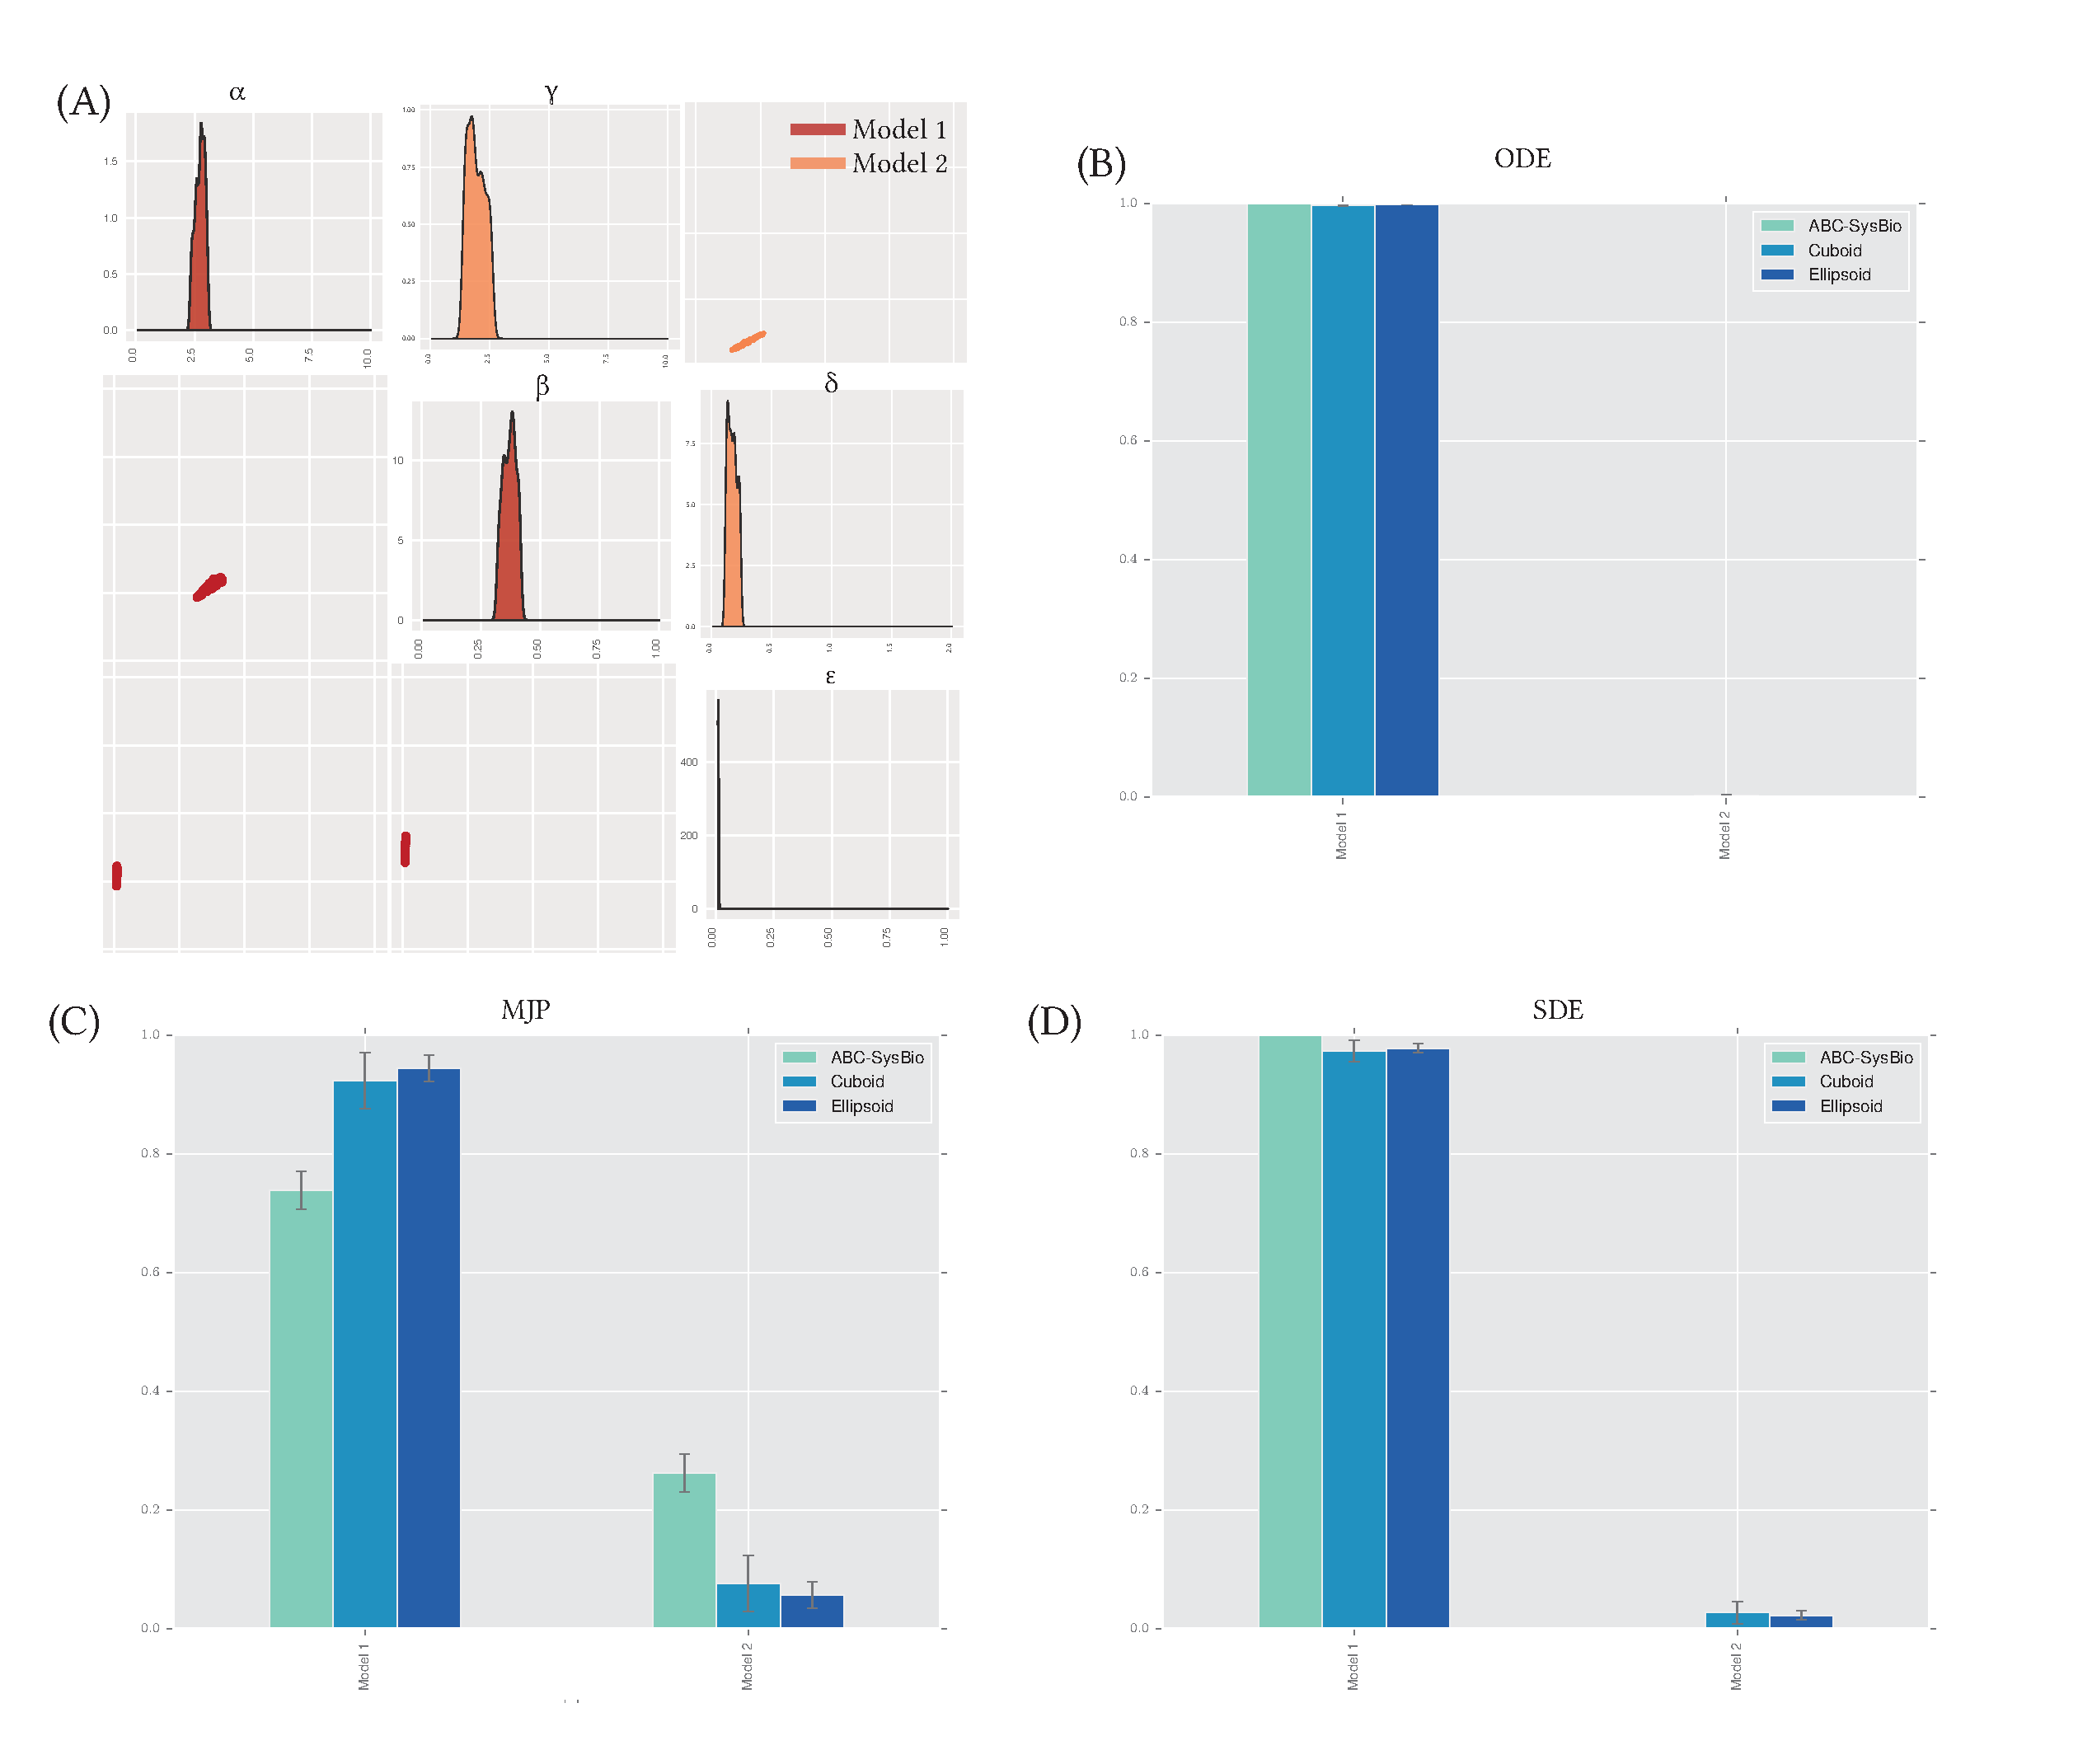
\includegraphics[width=\textwidth]{chapterStabilityFinder/images/ex1_sum.png}
\caption[LoF caption]{\label{fig:rob_sysbio1}: Robustness analysis of the three models for the spread of infectious diseases. (A-C) The posterior distributions of the three models compared. (D) I use three methods to calculate robustness, ABC-SysBio model selection, the volume of the hyper-cuboid approximation of the posterior distribution and the volume of the hyper-ellipsoid approximation of the posterior distribution. There is good agreement between all three methods. All three methods show that Model 1, the simplest model, is the most robust model. }

\end{center}
\end{figure*}
\clearpage

\subsection{Case study 2: Population growth}

The second example I will use to demonstrate the effectiveness of the method used here for robustness calculation is a population growth model.

The data was obtained by simulating an immigration-death model (XXX). Then this model and a model of logistic growth are compared for robustness of their posterior distributions. 
Model 1:
\begin{align*}
  \frac{dI}{dt} &= \alpha - \beta I
\end{align*}
Model 2:
\begin{align*}
  \frac{dI}{dt} &= \gamma - I	(\delta - \epsilon I)
\end{align*}


{\color{red} check these equations}

As done in Section~\ref{sec:cs1}, two analyses were done on these two models. First, ABC-SysBio model selection was used to find the most robust model. Then parameter inference was done on each model. The resulting posterior distributions (shown in Figure~\ref{fig:rob_sysbio4}), were compared for robustness using the cuboid and the ellipsoid approximation methods. All three robustness measures find that Model 1 is the most robust model. The analysis was repeated for~\acrshort{ode},~\acrshort{mjp} and~\acrshort{sde} simulations, all arriving to the same result of Model 1 being the most robust. The results are shown in Figure~\ref{fig:rob_sysbio4}.


\begin{figure*}[p]
\begin{center}
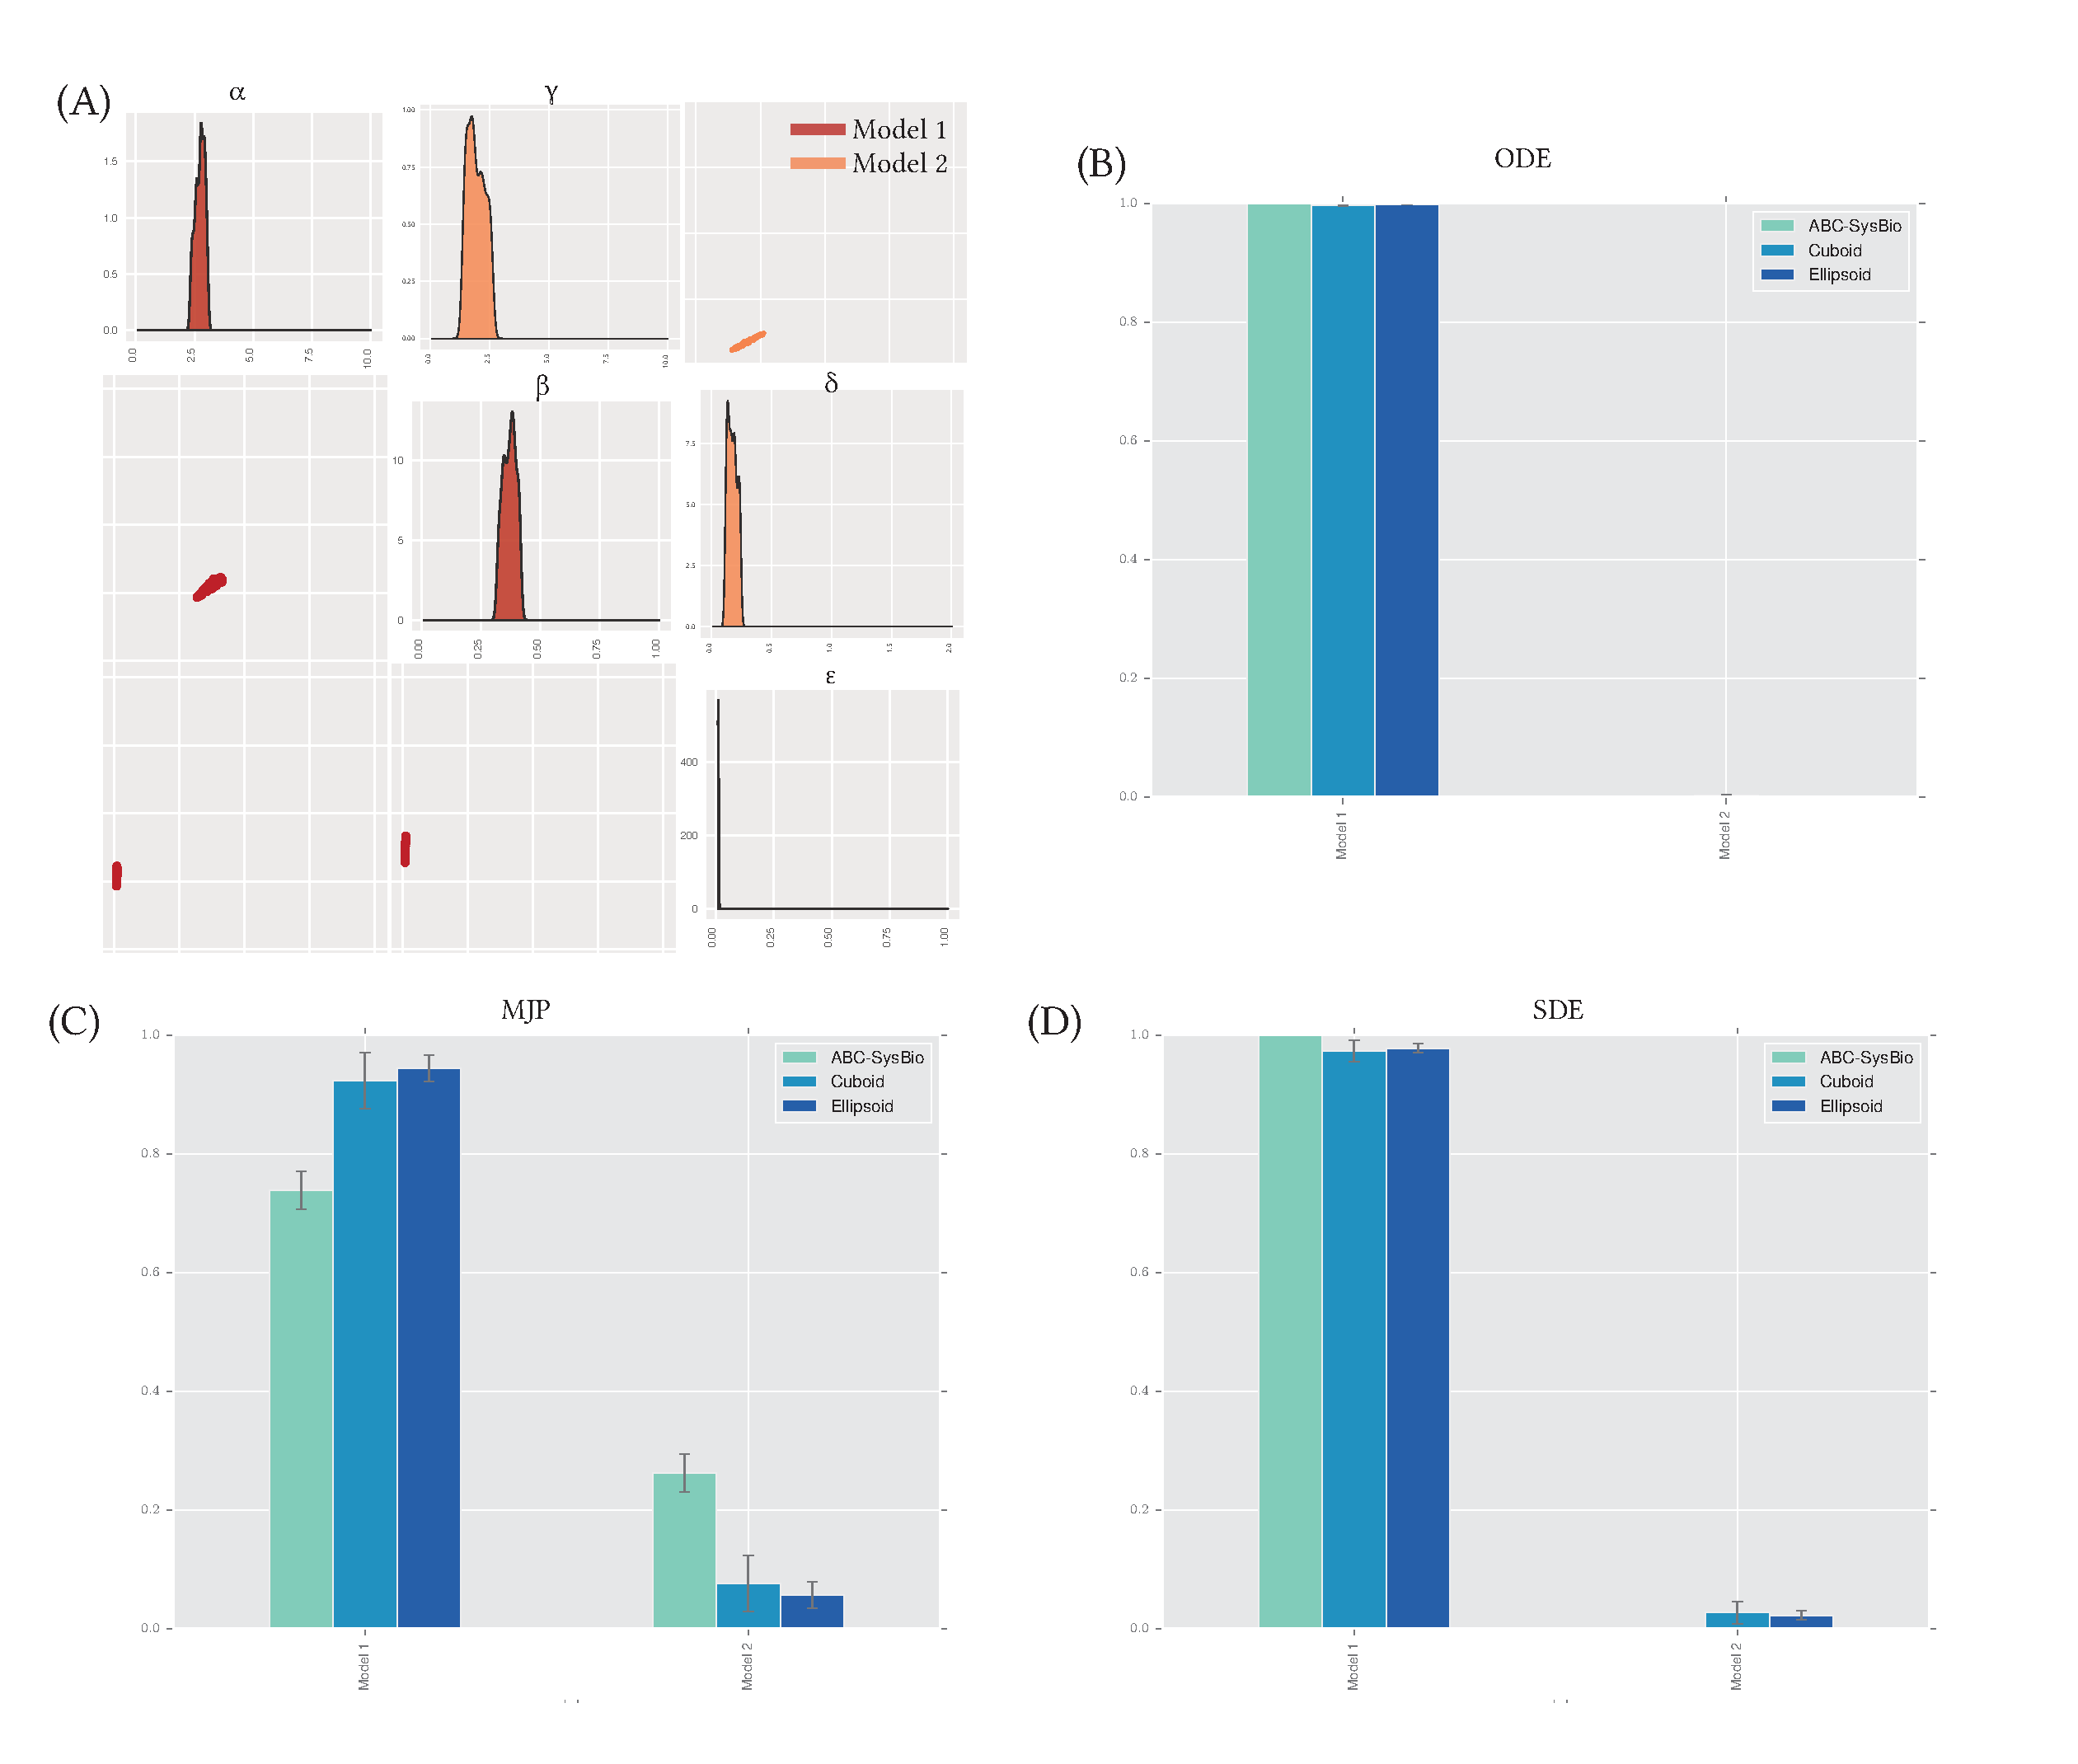
\includegraphics[width=\textwidth]{chapterStabilityFinder/images/ex4_summ.png}
\caption[LoF caption]{\label{fig:rob_sysbio4}: Robustness comparison of two population growth models. (A) The posterior distributions of the two models. (B-D) The models were simulated using \acrshort{ode},~\acrshort{mjp} and~\acrshort{sde}. Both the cuboid and the ellipsoid approximations agree with ABC-SysBio model selection results. }
\end{center}
\end{figure*}

\clearpage


The two case studies used above show that the hyper-cuboid and the hyper-ellipsoid approximation of model robustness agree with the results obtained from ABC-SysBio model selection. 

The drawbacks of our method compared to model selection are that each model stability analysis must reach completion in order to be used. In Bayesian model selection, where model selection is incorporated in the process, each model is also considered a particle (XXX) with an associated weight. If a model is performing poorly it does not proceed in the algorithm and is dropped when the weight falls low enough so that the model is not sampled (XXX). This can save time in the analysis as computational resources are not wasted on models that perform the required behaviour poorly. Using StabilityFinder for model selection, we will inevitably fall in this problem, since each model must reach the given final \textepsilon{} in order to be comparable. This means that time will be spent in running models that are potentially a bad fit, or that have posteriors so small compared to the prior that it will take a long time for StabilityFinder to find it. This is a compromise we make in order to be able to run the models separately, as model selection is not the primary purpose of this software. 

Even though this method of calculating robustness requires all the models' parameter inference to come to completion, the results still agree with ABC-SysBio model selection where that is not required (see Figures~\ref{fig:rob_sysbio1} and \ref{fig:rob_sysbio4}).


\section{Applications of StabilityFinder}

In this section we apply StabilityFinder to switch models in order to find the design principles underlying their stabilities. First we apply it to a simple model with known results, the \textcite{Gardner:2000vha} toggle switch. This allows us to test StabilityFinder before applying it to further models.

\subsection{Testing StabilityFinder}

\textcite{Gardner:2000vha} constructed the first synthetic genetic toggle switch~\autocite{Gardner:2000vha}. Their model consisted of two mutually repressing transcription factors, as shown in Figure~\ref{fig:fig2}A, and in the deterministic case is defined by the following \acrshort{ode}s.

\begin{align*}
\frac{du}{dt} &= \frac{a_1}{1+v^{\beta}} - u\\
\frac{dv}{dt} &= \frac{a_2}{1+u^{\gamma }} - v,
\end{align*}

\noindent where \textit{u} is the concentration of repressor 1, \textit{v} the concentration of repressor 2, $a_1$ and $a_2$ denote the effective rates of synthesis of repressors 1 and 2 respectively, \textbeta{} is the cooperativity of repression of promoter 1 and \textgamma{}of repressor 2. Gardner \textit{et al} studied the deterministic case and concluded that there are two conditions for bistability for this model; that $a_1$ and $a_2$ are balanced and that \textbeta{}, \textgamma{}\textgreater 1 \autocite{Gardner:2000vha}. In order to test StabilityFinder we used it to find the posterior distribution for which this model exhibits bistable behaviour. We therefore set the desired behaviour to two steady states, and using a wide range of values as priors as shown in Table~\ref{tab:gard_det_stoch}, we used StabilityFinder to find the parameter values necessary for bistability to occur. The posterior distribution calculated by StabilityFinder for the Gardner deterministic case is shown in Figure~\ref{fig:gard_mod}B.

\begin{table}[htbp]
\centering
\caption{Gardner switch priors in the deterministic and stochastic cases}
\label{tab:gard_det_stoch}
\begin{tabular}{@{}cccccc@{}}
\toprule
\multicolumn{4}{c}{Parameters}                          & \multicolumn{2}{c}{Species} \\ \cmidrule(lr){1-4}
\cmidrule(lr){5-6}
$a_1$ & $\beta$ & $a_2$ & \multicolumn{1}{c}{$\gamma$} & $s_1$        & $s_2$        \\
0-60  & 0-5     & 0-60  & 0-5                           & 0-100        & 0-100        \\ \bottomrule
\end{tabular}
\end{table}

These results agree with the results reported by~\textcite{Gardner:2000vha}~\autocite{Gardner:2000vha}. For this switch to be bistable $a_1$ and $a_2$ must be balanced while \textbeta{} and \textgamma{} must both be \textgreater 1, as can be seen in the marginal distributions of \textbeta{} and \textgamma{} in Figure~\ref{fig:fig2}B. The conditions set by the original paper for parameters $a_1$ and $a_2$ are met. 

We next applied StabilityFinder to the case of the Gardner switch under stochastic dynamics using the same priors as the deterministic case, and again searched the parameter space for bistable behaviour. The posterior is shown in Figure~\ref{fig:gard_mod}C. We can see that the conditions on the parameters required for bistability in the deterministic case generally still stand in the stochastic case. There appears to be slightly looser requirements on the parameters of the stochastic model (wider marginal distributions), which is expected due to the nature of clustering deterministic steady states versus stochastic steady states. The gap statistic is used in the case of the stochastic case, as it is capable of dealing with noisier data whereas a simpler and faster algorithm is used for clustering the deterministic solutions. These results demonstrate that StabilityFinder can be used to find the parameter values that can produce a desired stability and allow us to confidently apply the methodology to more complex models.


\begin{figure*}[htbp]
\begin{center}
	\includegraphics[scale=0.8]{chapterStabilityFinder/images/gardner_model.png}
	\caption[LoF caption]{\label{fig:gard_mod}}
\end{center}
\end{figure*}

\begin{figure*}[htbp]
\begin{center}
	\includegraphics[scale=0.8]{chapterStabilityFinder/images/gardner_posteriors.png}
	\caption[LoF caption]{\label{fig:gard_post}}
\end{center}
\end{figure*}
\clearpage
%\begin{figure*}[h]
%\begin{center}
%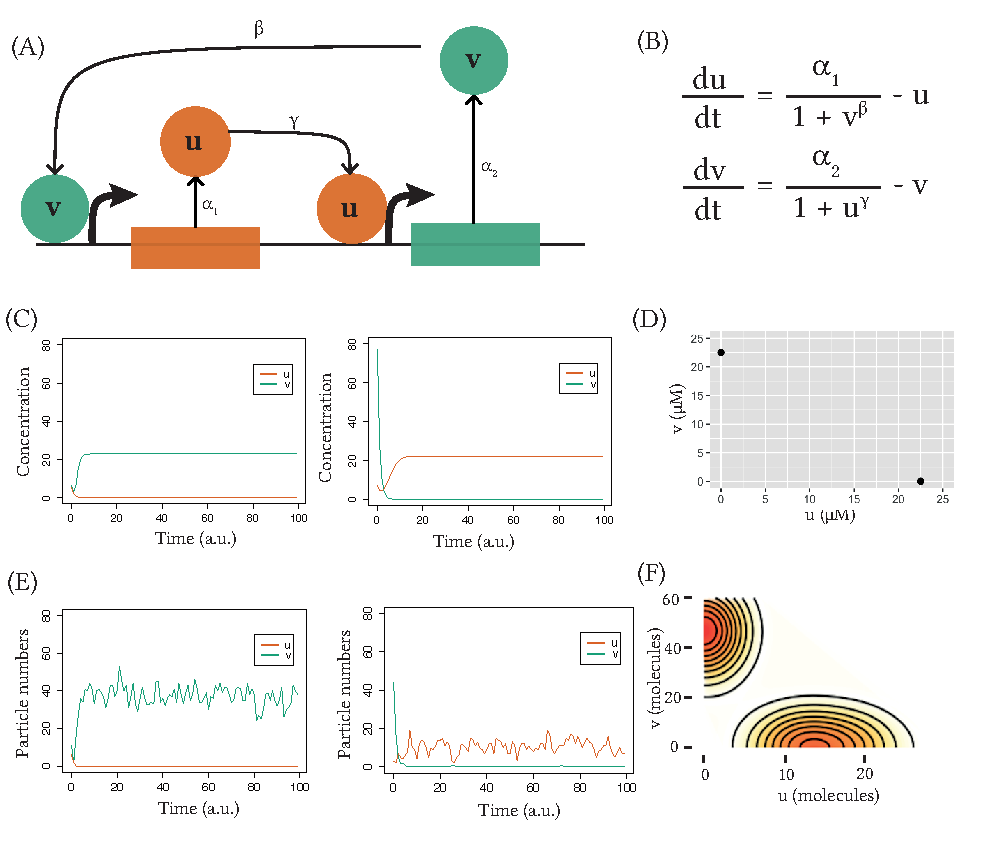
\includegraphics[width=\textwidth]{chapterStabilityFinder/images/gardner_poster.png}
%\caption[LoF caption]{ \label{fig:fig2}: Elucidating the stability of the Gardner switch. The Gardner model (A) consists of two mutually repressing transcription factors. It can be reduced to a two-equation system, where $u$ and $v$ are the two transcription factors, $a_1$,$a_2$ are their effective rates of synthesis, $u$,$v$ are their concentrations and $\beta$, $\gamma$ represent the cooperativity of each promoter. There are four parameters in the model, for which we want to find the values for which this system is bistable. We use StabilityFinder to find the posterior distribution of the bistable Gardner switch, deterministically (B) and stochastically (C). The posterior distributions are shown as the density plots of each parameter as well as each one plotted against the other. }
%\end{center}
%\end{figure*}
%\clearpage


\subsection{Lu toggle switch models}

We next analyzed an extension of the Gardner switch model developed by~\textcite{Lu:2014kc}~\autocite{Lu:2014kc}. They considered two types of switches, the classic switch consisting of two mutually repressing transcription factors (model \acrshort{cs-lu}), as well as a \acrfull{dp-lu}.  The classical switch was found to be bistable given the set of parameters used, while the DP switch was found to be tristable~\autocite{Lu:2014kc}. The classical model used in their study is given by the following system of \acrshort{ode}s.

\begin{align*}
\dot{x} & = g_{x}\, H^{S}_{xy}(y) -k_{x}x \\
\dot{y} & = g_{y}\,H^{S}_{yx}(x) -k_{y}y,
\end{align*}
where
\begin{align*}
H^{S}_{I}(x) &= H^{-}_{I}(x)+\lambda_{I}H^{+}_{I}(x) \\
H^{-}_{I}(x) &= 1 \big/\left[1+(x/x_{I})^{n_{I}}\right] \\
H^{+}_{I}(x) &= 1-H^{-}_{I}(x),
\end{align*}

\noindent and $g_I$ represents the production rate, $k_I$ the degradation rate, $n_I$ the Hill coefficient, $x_I$ the Hill threshold concentration and $\lambda_I$ the fold change of the transcription rates, and $I\in\{xy, yx, xx, yy\}$. 

For the parameter values used in the Lu study, the classical switch exhibits three steady states (Figure~\ref{fig:fig3}), two of which are stable and one is unstable. Using StabilityFinder with priors centred around the parameter values used in the original paper (see Supplementary Information), we can identify the most important parameters for achieving bistability. The posterior distribution of these models are shown in Figure~\ref{fig:fig3}A. We find that the parameters representing the rates of degradation of the transcription factors in the system ($k_x$,$k_y$) must both be large in relation to the prior ranges for bistability to occur. Protein degradation rates have been shown to be important for many system behaviours including oscillations \autocite{XXX}. StabilityFinder


\begin{figure*}[htbp]
\begin{center}
	\includegraphics[scale=0.5]{chapterStabilityFinder/images/lu_bifurc.png}
	\caption[LoF caption]{\label{fig:lu_bifurc}  Stream plot of the vector plot of the (A) \acrshort{cs-lu} and \acrshort{dp-lu} switches. The colours indicate the magnitude of the vectors, with yellow indicating high and red low values. The blue points represent stable steady states and the grey points represent unstable steady states.  }
\end{center}
\end{figure*}




It is known that that the addition of positive autoregulation to the classical toggle switch can induce tristability  \autocite{XXX, Lu:2014kc}. Here we investigate the interplay of positive autoregulation on the values of the other parameters in the model. We extended the analysis presented in ~\textcite{Lu:2014kc} by including the switch with single positive autoregulation (model \acrshort{sp-lu}), where an asymmetry of positive feedbacks is present between the two genes. The advantage of using StabilityFinder over solving the system analytically is that the full parameter space is explored rather than solving the system for a single set of parameters. This allows us to deduce model properties that could not otherwise be identified. Robustness to parameter fluctuations can be explored, as well as parameter correlations and restrictions on the values they can take while still producing the desired behaviour.  

The \acrshort{dp-lu} model is given by
\begin{align*}
\dot{x} = f_{x}(x,y) &= g_{x}\, H^{S}_{xy}(y)\, H^{S}_{xx}\,(x)-k_{x}x \\
\dot{y} = f_{y}(x,y) &= g_{y}\,H^{S}_{yx}(x)\,H^{S}_{yy}\,(y)-k_{y}y,
\end{align*}
whereas the \acrshort{sp-lu} switch is modelled using the following \acrshort{ode} system
\begin{align*}
\dot{x} & = g_{x}\, H^{S}_{xy}(y)\, H^{S}_{xx}\,(x)-k_{x}x \\
\dot{y} & = g_{y}\,H^{S}_{yx}(x) - k_{y}y.
\end{align*}


\begin{figure*}[htbp]
\begin{center}
	\includegraphics[width=\textwidth]{chapterStabilityFinder/images/LU_diagrams.png}
	\caption[LoF caption]{\label{fig:lu_mods} The three LU toggle switch models. (A) \acrshort{cs-lu}, (B) \acrshort{sp-lu} and (C) \acrshort{dp-lu}.   }
\end{center}
\end{figure*}



\begin{table}[htpb]
\centering
\caption{Priors of the classical(\acrshort{cs-lu}), single positive (\acrshort{sp-lu}) and double positive (\acrshort{dp-lu}) models.}
\label{tab:lu_all}
\begin{tabular}{@{}ccccc@{}}
\toprule
Parameter                                            & Symbol & \acrshort{cs-lu}       & \acrshort{sp-lu}        & \acrshort{dp-lu}       \\ \midrule
\multirow{2}{*}{Production rate}                & gx        & 30-50   & 1-2       & 1-100    \\
                                                & gy        & 30-50   & 20-25     & 1-100    \\[4pt]
\multirow{2}{*}{Degradation rate}               & kx        & 0-0.5   & 50-55     & 0-1      \\
                                                & ky        & 0-0.5   & 48-52     & 0-1      \\[4pt]
\multirow{2}{*}{Hill coefficient}               & nxy       & 1-5     & 30-35     & 0-10     \\
                                                & nyx       & 1-5     & 0.1-0.2   & 0-10     \\[4pt]
\multirow{2}{*}{Hill thresholds concentration}  & xxy       & 100-300 & 2-3       & 100-1000 \\
                                                & xyx       & 100-300 & 0.4-0.6   & 100-1000 \\[4pt]
\multirow{2}{*}{Transcription rate fold change} & lxy       & 0-0.5   & 0.02-0.04 & 0-1      \\
                                                & lyx       & 0-0.5   & 0.02-0.04 & 0-0.2    \\[4pt]
\multirow{2}{*}{Hill coefficient}               & nXX       & -       & 25-30     & 0-10     \\
                                                & nYY       & -       & 0.01-0.02 & 0-10     \\[4pt]
\multirow{2}{*}{Hill thresholds concentration}  & xXX       & -       & 0.4-0.5   & 50-500   \\
                                                & xYY       & -       & 1-3       & 50-500   \\[4pt]
\multirow{2}{*}{Transcription rate fold change} & lXX       & -       & 65-72     & 1-20     \\
                                                & lYY       & -       & 0.02-0.04 & 1-20     \\ \hline
\end{tabular}
\end{table}

\noindent We find that the switch with single positive autoregulation is capable of bistable behaviour as seen in Figure~\ref{fig:fig3}B, but this is only possible when the strength of the promoter under positive autoregulation, $gx$, is small. There appear to be no such constraints on the strength of the original, unmodified, promoter, $gy$.  

Upon examination of the \acrshort{dp-lu} model, we also find that tristability in the switch is relatively robust, as tristability is found across a large range of parameter values, with no parameters strongly constrained. Two types of tristable behaviour are identified, one where the third steady state is at (0,0) and and one where the third steady state has non-zero values. This result agrees with previous work by~\textcite{Guantes:2008gs}, who found that a switch can exhibit two kinds of tristability, one in which the third steady state is high (\RNum{3}$_H$) and one in which it is low (\RNum{3}$_L$)~\autocite{Guantes:2008gs}. %The difference between the two tristable switches is explored in a later section. 

deterministic dynamics~\autocite{Guantes:2008gs}. The classical switch is also capable of both bistable and tristable behaviour when stochastic dynamics capture small number effects~\autocite{Ma:2012dt}. It is therefore of great interest to understand the conditions under which these two behaviours occur in both stochastic and deterministic scenarios. 

In order to do this using StabilityFinder, we first obtained posterior distributions for bistable and tristable behaviours in the deterministic case (\acrshort{dp-lu} model) and then compared the individual parameter distributions (Figure~\ref{fig:fig6} and Supplementary Information). From analysis of the one dimensional marginal distributions it appears that there is no difference in the parameter values that allow a switch to be bistable versus tristable (Figure~\ref{fig:fig6}B). However, upon examination of the two dimensional marginal distributions we find that the correlation structure of a small subset of the posterior parameter values is in fact different under the two behaviours (Figure~\ref{fig:fig6}C). Most notably, we find differences in the bivariate distribution of the two parameters for gene expression, $gx$ and $gy$, as highlighted in Figure~\ref{fig:fig6}C, box 1. In the tristable case the distribution is more constrained than in the bistable case, as both parameters must be small for tristability to arise. 


\begin{table}[htpb]
\centering
\caption{Priors used in the three-node switch}
\label{tab:multi_priors}
\begin{tabular}{@{}ccc@{}}
\toprule
Parameter                           & Symbol & Range   \\ \midrule
Production rate                & gx        & 3-5    \\
Degradation rate               & kx        & 0-0.2     \\
Hill coefficient               & nxy       & 0-2    \\
Hill thresholds concentration  & xxy       & 140-160 \\
Transcription rate fold change & lxy       & 0-0.2     \\
Hill coefficient               & nxx       & 2-4     \\
Hill thresholds concentration  & xxx       & 90-110  \\
Transcription rate fold change & lxx       & 8-12    \\ \bottomrule
\end{tabular}
\end{table}


\begin{figure*}
	\begin{center}
		\includegraphics[width=\textwidth]{chapterStabilityFinder/images/Lu_234.png}
		\caption[LoF caption]{ \label{fig:lu_234}:}% Design principles of a tristable switch. (A) Using the Lu model with added positive autoregulation we uncover the design principles dictating if a switch will be bistable or tristable. (B) By considering each parameter separately we cannot find a significant difference in the parameter values acceptable for a bistable versus a tristable switch. (C) By considering the bivariate distributions of the parameters we can uncover the differences in the parameters of a bistable switch compared to a tristable switch. The posterior distribution of the bistable switch is shown in red and of the tristable switch in blue. The bivariate distributions for which a difference is observed between a bistable and a tristable switch are in black boxes. }
	\end{center}
\end{figure*}


%\begin{figure*}[h]
%\begin{center}
%\includegraphics[width=\textwidth]{chapterStabilityFinder/images/Lu_bi_tri_design_princ.png}
%\caption[LoF caption]{ \label{fig:fig6}: Design principles of a tristable switch. (A) Using the Lu model with added positive autoregulation we uncover the design principles dictating if a switch will be bistable or tristable. (B) By considering each parameter separately we cannot find a significant difference in the parameter values acceptable for a bistable versus a tristable switch. (C) By considering the bivariate distributions of the parameters we can uncover the differences in the parameters of a bistable switch compared to a tristable switch. The posterior distribution of the bistable switch is shown in red and of the tristable switch in blue. The bivariate distributions for which a difference is observed between a bistable and a tristable switch are in black boxes. }
%\end{center}
%\end{figure*}
\clearpage

Parameters $xYY$ and $gy$ are tightly constrained in the tristable case and both required to be small, but less so in the bistable case (Figure~\ref{fig:fig6}C, box 3). Another notable difference is between parameters $xXX$ and $lXX$ shown in Figure~\ref{fig:fig6}C, box 4, where they are constrained in the bistable case but not the tristable case. Interestingly, we also find parameter correlations conserved between the bistable and tristable case, as seen in Figure~\ref{fig:fig6}C, box 2, where parameters $lXX$ and $gx$, positive autoregulation and gene expression are negatively correlated in both cases.  This highlights the importance of treating unknown parameters as distributions rather than fixed values when studying the parameter values of a model, as they are capable of uncovering not only the ranges and values needed but also the correlations between parameters that would not have otherwise been detected.

To further demonstrate the flexibility of our framework we investigated a system capable of higher stabilities. Multistability is found in differentiating pathways, like the myeloid differentiation pathway~\autocite{Ghaffarizadeh:2014bt, Cinquin:2005go}. We allow for these more complex dynamics by extending the Lu DP model by adding another gene, making it a three gene switch.  This new system is depicted in Figure~\ref{fig:fig8}A. In StabilityFinder we look for six steady states, the output being in nodes $X$ and $Y$ and using the priors shown in Table~\ref{tab:multi_priors}. We successfully find that the system is capable of six steady states, as shown in Figure~\ref{fig:fig8}C and as predicted mathematically and shown in Figure~\ref{fig:fig8}B. Interestingly, and consistent with the results presented above, we find that the most constrained parameters for this behaviour are again the degradation rate of the proteins, $kx$. Additionally we find that the Hill coefficients for the repressors, $nxy$, are tightly contrained to be smaller than 1.5 as seen in Figure~\ref{fig:fig8}D. This example demonstrates that Stability Finder can be used to elucidate the dynamics of more complex network architectures, which will be key to the successful design and construction of novel gene networks as synthetic biology advances.

\begin{figure*}[h]
\begin{center}
\includegraphics[scale=0.6]{chapterStabilityFinder/images/lu_6ss.png}
\caption[LoF caption]{ \label{fig:fig8}: The three-node mutual repression model, with added positive auto-regulation on each node. (A) The model. The model is studied in two dimensions using StabilityFinder, $X$ and $Y$. (B) The phase plot of the resulting final population of StabilityFinder. There are 6 steady states. (C) The posterior distribution of the 6-steady state three-node system. Parameters $kx$ and $nxy$ are the most constrained.}
\end{center}
\end{figure*}




\begin{figure*}[p]
\begin{center}
\includegraphics[width=\textwidth]{chapterStabilityFinder/images/lu_paper_post.png}
\caption[LoF caption]{ \label{fig:fig3}: The three variants of the Lu models. (A)\textbf{CS (deterministic).}  The classic switch with no autoregulation is bistable. The most restricted parameters for this behaviour are $kx$ and $ky$ which both have to be high relative to the prior while the net protein production for $X$ and $Y$ myst be balanced. (B)\textbf{SP (deterministic).}The extended Lu model with a single positive autoregulation on $X$. This model is bistable when $gx$ is small. (C) \textbf{DP (deterministic).} The Lu model with double positive autoregulaiton is tristable, and its posterior distribution shown here. We find two types of tristable behaviour, one where the third steady state is zero-zero and one where the third state is high (non-dead).}
\end{center}
\end{figure*}
\clearpage




\subsection{Mass Action switches}						
Although the DP switch can achieve tristability, we investigated how the addition of positive autoregulation alters the robustness of the switch for bistable behaviour. Here we define a robust system as a device that can withstand fluctuations in parameter values and still produce the desired behaviour (parametric robustness). Feedback loops are well known key regulatory motifs~\autocite{Brandman:2005ci}. Although negative feedback loops are essential for homeostasis and buffering~\autocite{Thomas:1995id} and can increase robustness to extrinsic noise sources, we focussed on the addition of positive feedback because this has been shown to increase robustness in other systems \autocite{XXX}. We use StabilityFinder to compare the two models, and determine whether its worthwhile building a bistable circuit with added positive feedback.
%StabilityFinder allows us to study more complex systems and to take stochasticity into account. This is relevant in a biological systems in which realistic models tend to involve many species and interactions and where small molecule numbers and external noise are non negligible. 

In order to study the switch system in the most realistic way, we avoid using the quasi-steady state approximation (QSSA) that is often used in modelling the toggle switch. Using mass action, this changes the two-equation system used in~\textcite{Lu:2014kc}~\autocite{Lu:2014kc} into a system of 18 equations and 7 parameters in the classical switch case. These are shown in the Supplementary Information.% Using mass action, the two models representing the  C switch with no autoregulation and DP switch are shown in Figure~\ref{fig:fig4} {\color{red} No they're not}.  

\begin{figure*}[htbp]
\begin{center}
\includegraphics[scale=0.4]{chapterStabilityFinder/images/MA_QSSA.png}
\caption[LoF caption]{ \label{fig:fig5}: (A) Separating transcription and translation in the mass action model. (B) Transcriptional bursting does not allow for a bistable switch. (C) The Quassi Steady state approximation assumption that the dimerization reaction ($dim$) is much faster than its reverse ($dim\_r$) cannot be justified here. The median of the data (red) lies below the x=1 line (black dashed line) which indicates that in the majority of the particles in the posterior $\frac{dim}{dim\_r} < 1$  (D) No difference was found in the robustness to parameter fluctuations for the two models tested here.}
\end{center}
\end{figure*}
\clearpage


Given the posterior distributions shown in Figure~\ref{fig:fig4}, we find that the parameter for transcription factor degradation ($deg$) has to be high, a result that reflects the findings for the Lu models above {\color{red} Do we really see that??}. We also find that the addition of positive feedback loops greatly increases the system's robustness to parameter fluctuations as seen in Figure~\ref{fig:fig4}D. Adding positive feedback loops to the model allows it to be bistable over a greater range of parameter values, but only when the system is symmetric. When this constraint is removed we no longer see a difference in robustness between the CS-MA and DP-MA models. {\color{red} What does this mean? }



%This indicates that small fluctuations in parameters in the cellular environment will not affect the system's ability to be bistable, and thus makes it more suitable for use in synthetic biological applications where a very constrained parameter set can be too restrictive.% This makes it a better candidate for building new synthetic devices based on the toggle switch design.

%We identified the parameter region within which these models are bistable, information that is important when building such a device in the lab. In the future, by selecting the system components accordingly, the parameter values can be adjusted \textit{in vivo}. For example, the desired level of gene expression can be accomplished by selecting the appropriate RBS sequence~\autocite{Salis:2009gk}. Another method to modify the parameter values \textit{in vivo} is to select the promoter to have the strength corresponding to the levels of gene expression and repression desired. Activity of each promoter can be measured and standardised~\autocite{Kelly:2009bj} making this process possible. For a system requiring more than one promoter, these can be efficiently selected from a promoter library using a genetic algorithm~\autocite{Wu:2011bq}. These standardised interchangeable components with known sequence and activity~\autocite{Kelly:2009bj,Canton:2008fv} can be selected and used to construct a desired system and replicate the parameter values found using StabilityFinder.

We find that in the stochastic case, both the simple switch, S-MA, and positive autoregulation switch, DP-MA, are capable of both bistable and tristable behaviour. The fact that tristability can occur in the classical model is consistent with the effect of small molecule numbers; if gene expression remains low, it provides the opportunity for small number effects to be observed, and the third steady state to stabilise \autocite{Ma:2012dt}. In order to ensure that the tristable switches found in the stochastic case are truly tristable, we re-sample the posterior distributions and simulate to steady state. If the resulting phase plots are tristable then we know that the posterior truly represents tristability. As can be seen in Figure~\ref{fig:fig7}B, differences in the parameter values are observed between the bistable and tristable switches, in both CS-MA and DP-MA models. The design principles for both the CS-MA model and the DP-MA model are summarised in Table~\ref{tab:des_prin}

\begin{table}[]
\centering
\caption{Design principles of bistable and tristable switches}
\label{tab:des_prin}
\begin{tabular}{@{}ccccc@{}}
\toprule
                    & \multicolumn{2}{c}{\textbf{CS-MA}} & \multicolumn{2}{c}{\textbf{DP-MA}} \\ \cmidrule(l){2-3}\cmidrule(l){4-5}
                    & \textit{Bistable}    & \textit{Tristable}   & \textit{Bistable}    & \textit{Tristable}   \\\cmidrule(l){2-2}\cmidrule(l){3-3}\cmidrule(l){4-4}\cmidrule(l){5-5}
dimerisation        & High        & Low         & High        & Low         \\
protein degradation & -           & -           & -           & Low         \\
dimer degradation   & Low         & -           & Low         & -           \\\bottomrule
\end{tabular}
\end{table}


\begin{figure*}[h]
\begin{center}
\includegraphics[scale=0.5]{chapterStabilityFinder/images/MA_sym_post.png}
\caption[LoF caption]{ \label{fig:fig4}: Adding positive feedback increases robustness to parameter fluctuations. We compare the posterior distributions of the simple mass action switch and the switch with added double positive autoregulation (A). The two models were both capable of bistable behaviour (B). The two posterior distributions are shown in (C). Comparing the functional region $F$ of the posterior distributions (D) we find that there is a five-fold increase in robustness when positive autoregulation is added. This is not the case for the asymmetric switch in which there is no significant difference in robustness between the CS-MA and DP-MA models.}
\end{center}
\end{figure*}
\clearpage

\begin{figure*}[h]
\begin{center}
\includegraphics[scale=0.5]{chapterStabilityFinder/images/MA_stoch_design_princ.png}
\caption[LoF caption]{ \label{fig:fig7}: Tristability is possible in the mass action toggle switch models only when simulated stochastically. (A) the simple toggle switch with no autoregulation can be both bistable and tristable. The two posteriors are shown, where the posterior distribution of the bistable switch is shown in red and of the tristable switch in blue. From the posterior distribution we can deduce the the dimerization parameter must be small for tristability to occur but large for bistability. The switch with double positive autoregulation and its posterior distributions for the bistable and tristable case are shown in (B). A sample phase plot of a stochastic tristable and bistable mass action switch is shown in (C). Comparing the robustness of the switch with and without positive autoregulation, we don't find a significant difference (D).}
\end{center}
\end{figure*}

\section{Discussion}




We have developed an algorithm that can identify the parameter regions necessary for a model to achieve a given number of stable steady states. The novelty in our framework over existing methodology is that complex models can be analyzed assuming both deterministic and stochastic dynamics. We have shown that the algorithm can be used to infer parameter ranges and compare robustness between models. We found that adding positive feedback increases the robustness of a toggle switch model to parameter fluctuations. We also found that stochastic modelling can enable a model to achieve stabilities not possible in the deterministic case. We uncovered the design principles that make a tristable switch and finally we found that a three-node switch is capable of hexastability.

Tools that can identify parameter regions that give rise to specific behaviours will be key for the success of synthetic biology. In the future, by selecting the system components accordingly, the parameter values can be adjusted \textit{in vivo}. For example, the desired level of gene expression can be accomplished by selecting the appropriate RBS sequence~\autocite{Salis:2009gk}. Another method to modify the parameter values \textit{in vivo} is to select the promoter to have the strength corresponding to the levels of gene expression and repression desired. Activity of each promoter can be measured and standardised~\autocite{Kelly:2009bj} making this process possible. For a system requiring more than one promoter, these can be efficiently selected from a promoter library using a genetic algorithm~\autocite{Wu:2011bq}. These standardised interchangeable components with known sequence and activity~\autocite{Kelly:2009bj,Canton:2008fv} can be selected and used to construct a desired system and replicate the parameter values found using StabilityFinder.

The methodology presented here can also be used to study the topology of more complex multistable switches that exist in natural biological systems such as developmental pathways. We also limited our framework to the objective behaviour of a given number of stable steady states. This could be extended to examine systems with a given switching rate or systems robust to a particular set of perturbations, both of which could be of great importance for building more complex genetic circuits.

More generally our results highlight that changing the level of abstraction included in the model can significantly alter the observed multistationarity. This is further exacerbated by a change in the dynamics from deterministic to stochastic. These results for the case of multistationarity, assuming they translate to systemic behaviour more generally, suggest that a programme of experimental work, combined with systems modelling, is required to understand the rules of thumb for abstraction in model based design of synthetic biological systems.   


\section{Summary}

In this chapter...
